%!TEX program = xelatex
\documentclass[cn,hazy,blue,14pt,screen,device=normal]{elegantnote}
\usepackage{multirow}
\usepackage{enumitem}

\title{物理层; 概述}

\author{李聪聪}
\institute{3GPP TS 38.201 V15.0.0}

\version{0.1}
\date{\zhtoday}

\usepackage{array}

\begin{document}

\maketitle

\newpage
\tableofcontents
\newpage

\section{层 1 概述}
\subsection{与其他层的关系}
\subsubsection{协议架构}
 本规范中描述的无线电接口涵盖了用户设备(UE)和网络之间的接口。 无线接口由第1层,第2层和第3层组成。
 
 \begin{figure}[!hbp]
 	\centering
 	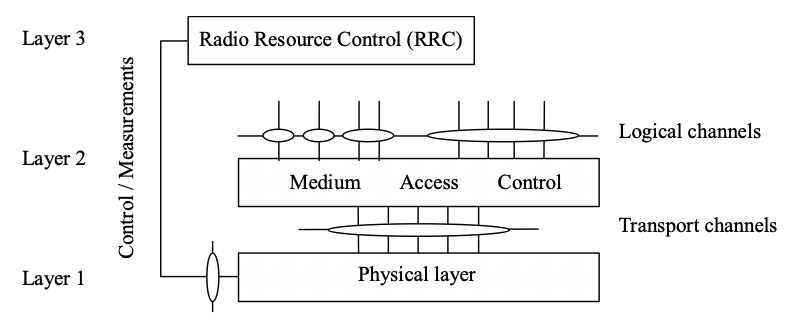
\includegraphics{Figure1Layers}
 	\caption{无线接口协议架构}
    \label{Figure1Layers}
 \end{figure}


如图 \ref{Figure1Layers} 所示,物理层连接着媒体访问控制层(Medium Access Control, MAC, 层 2)和无线资源控制层(Radio Resource Control, RRC, 层 3)。 不同层之间的圆圈表示服务访问点(Service Access Points, SAPs)。

物理层为 MAC 层提供了传输信道,而 MAC 层为 RRC 层提供了逻辑信道。不同逻辑信道上传输不同的数据,而不同的传输信道则规定了信息该如何通过空口进行传输。

物理层相关的规范参考 TS 38.200 系列。

MAC 层和 RRC 层相关规范参考 TS 38.300 系列。

\subsubsection{物理层为高层所提供的服务}
物理层为高层提供数据传输服务。MAC 层通过传输信道将需要发送的数据传递给物理层。详细内容可参考 3GPP TS 38.202: "NR; Services provided by the physical layer"。

\subsection{层 1 概述}
\subsubsection{多路访问}
NR物理层的多址方案基于具有循环前缀(CP)的正交频分复用(OFDM)。 对于上行链路,还支持带有CP的离散傅立叶变换扩频OFDM(DFT-s-OFDM)。 为了支持成对和非成对频谱的传输,同时使用了频分双工(FDD)和时分双工(TDD)。

为了使 NR 的物理层适应各种频谱分配,规定物理层以资源块(Resource Block, RB)为单位使用频谱资源。一个资源块包含 12 个相同间隔的子载波。

一个无线帧的持续时间为 10ms,包含 10 个子帧,子帧的持续时间为 1ms。每个子帧包括一个或多个时隙(slot),每个时隙包括 12/14 个符号(symbol)。关于帧结构的更多内容参考 3GPP TS 38.202: "NR; Services provided by the physical layer"。

\subsubsection{ 物理信道和调制 }
下行链路的物理信道包括以下几个:

\begin{itemize}[leftmargin=2cm]
	\item 物理下行链路共享信道(PDSCH)
	\item 物理下行链路控制信道(PDCCH)
	\item 物理广播信道(PBCH)
\end{itemize}

上行链路的物理信道包括以下几个:
\begin{itemize}[leftmargin=2cm]
	\item 物理随机接入信道(PRACH)
	\item 物理上行链路共享信道(PUSCH)
	\item 物理上行链路控制信道(PUCCH)
\end{itemize}

此外,还定义了主同步信号(Primary Synchronization Signal, PSS)、辅同步信号(Secondary Synchronization Signal, SSS)和参考信号(Reference Signal, RS)。

调制方案如下所示:

\begin{table}[!hbp]
	\resizebox{\textwidth}{12mm}{ 
		\begin{tabular}{|c|c|c|c|c|c|c|c|c|c|}
		\hline
         	& \multicolumn{4}{c|}{OFDM}                                                                         & \multicolumn{5}{c|}{DFT-s-OFDM}                             \\ \hline
			Downlink & \multirow{2}{*}{QPSK} & \multirow{2}{*}{16QAM} & \multirow{2}{*}{64QAM} & \multirow{2}{*}{256QAM} &                             &      &       &       &        \\ \cline{1-1} \cline{6-10} 
			Uplink   &                       &                        &                        &                         & $\pi / 2$-BPSK & QPSK & 16QAM & 64QAM & 256QAM \\ \hline
		\end{tabular}}
\end{table}

\end{document}
